\documentclass[bg-full]{resources/stylesheets/kult}
% \documentclass[bg-print]{resources/stylesheets/kult}
% \documentclass[bg-full, commercialfonts]{resources/stylesheets/kult}
% \documentclass[bg-print, commercialfonts]{resources/stylesheets/kult}

\usepackage%
[ backend=bibtex
, style=numeric
, citestyle=numeric
, sorting=ynt
]{biblatex}
\addbibresource{resources/bibliography.bib}
\usepackage{multicol}
\usepackage[notlof,notlot,nottoc]{tocbibind}
\usepackage{parskip}% needs to be after tocloft to not create a warning
\usepackage{pgffor, ifthen}
\newcommand{\notes}[3][\empty]{%
  \foreach \n in {1,...,#2}{%
    \ifthenelse{\equal{#1}{\empty}}
               {\rule{#3}{0.5pt}\\}
               {\rule{#3}{0.5pt}\vspace{#1}\\}
  }
}
\usepackage{rotating}
\usepackage{tikz}
\usetikzlibrary{shapes.geometric, snakes, mindmap}
\usepackage{amsmath}
\usepackage{newunicodechar}
\newfontface{\symbolfont}{Symbola}[Scale=MatchUppercase]
\NewDocumentCommand{\skull}{}{%
  \text{\symbolfont\symbol{"1F571}}%
}
\NewDocumentCommand{\ballot}{}{%
  \text{\symbolfont\symbol{"2610}}%
}
\newunicodechar{☐}{\ballot}
\usepackage{hyperref}
\hypersetup{
    colorlinks=true,
    linkcolor=KULTblue,
    citecolor=KULTblue,
    urlcolor=KULTblue,
    pdflinkmargin=-0.5pt,
    % pdfpagemode=FullScreen,
    bookmarksnumbered=true,
    linktoc=all,
    % hidelinks=true,
    pdfborder={0 0 0}
    }
\newcommand{\fld}[1]{\begin{Form}\TextField[bordercolor=,name=#1,backgroundcolor=,width=5mm,charsize=10pt]{\mbox{}}\end{Form}}
\newcommand{\checkbox}[1]{\scriptsize\begin{Form}\CheckBox[bordercolor=KULTblack,name=#1,backgroundcolor=,width=3mm]{\mbox{}}\end{Form}\normalsize}

\newcommand\gmnote[1]%
{\pgfsetfillopacity{0.30}\colorbox{black}%
{\pgfsetfillopacity{1}\parbox{\dimexpr\linewidth-2\fboxsep}{\strut \it \textbf{GM Note:~}#1\strut}}}
\newcommand{\KULTred}[1]{\textcolor{KULTred}{#1}}
\newcommand{\KULTgold}[1]{\textcolor{KULTgold}{#1}}
\newcommand{\KULTblue}[1]{\textcolor{KULTblue}{#1}}
\newcommand{\KULTrule}{\vspace*{1mm}\color{KULTblack}\hrule height 0.75mm\color{KULTtext}}

\covertext{%
  This is an \href{https://helmgast.se/en/meta/fan-content-policy}{\textbf{UNOFFICIAL}} module for
  \textit{KULT:~Divinity Lost}. It is not affiliated with and/or endorsed by Helmgast AB. A copy of
  the \href{https://kultdivinitylost.com/products/}{\textit{KULT: Divinity Lost} 4\textsuperscript{th} edition Core
  Rules} is required to play.
}
\usepackage{imakeidx}
\makeindex[intoc]
\indexsetup%
 { level=\section*,
   firstpagestyle=fancy
 }

\newcommand{\skilltree}[1]{% {{{
\scalebox{1.3}{%
\begin{tikzpicture}
\tikzstyle{common}=[draw=KULTgold, line width=0.7mm, inner sep=0pt, node distance=17mm]
\tikzstyle{passive}=[common, minimum size=12mm, diamond]
\tikzstyle{active} =[common, minimum size=10mm, circle]
\tikzstyle{albl}=[node distance=6.5mm, font=\scriptsize, minimum size=5mm]
\tikzstyle{plbl}=[node distance=7.5mm, font=\scriptsize, minimum size=5mm]
  \node[passive]                                   (will){\fld{will-#1}};
  \node[passive] at ( 1.7,-0.5)                    (refl){\fld{refl-#1}};
  \node[passive] at (-1.7,-0.5)                    (fort){\fld{fort-#1}};
  \node[active, below of=fort]                     (reas){\fld{reas-#1}};
  \node[active, below of=refl]                     (intu){\fld{intu-#1}};
  \node[active, below of=reas]                     (cool){\fld{cool-#1}};
  \node[active, below of=intu]                     (viol){\fld{viol-#1}};
  \node[active, below of=will, node distance=31mm] (perc){\fld{perc-#1}};
  \node[active, below of=perc]                     (char){\fld{char-#1}};
  \node[active, below of=char]                     (soul){\fld{soul-#1}};
  %
  \node[plbl, below of = will, label={[label distance=-2.5mm]below:{\tiny Keep it together}}]         (lblwill) {\textbf{Willpower}};
  \node[plbl, below of = refl, label={[label distance=-2.5mm]below:{\tiny Avoid Harm}}]               (lblrefl) {\textbf{Reflexes}};
  \node[plbl, below of = fort, label={[label distance=-2.5mm]below:{\tiny Endure Injury}}]            (lblfort) {\textbf{Fortitude}};
  \node[albl, below of = reas, label={[label distance=-2.5mm]below:{\tiny Investigate}}]              (lblreas) {\textbf{Reason}};
  \node[albl, below of = intu, label={[label distance=-2.5mm]below:{\tiny Read a Person}}]            (lblintu) {\textbf{Intuition}};
  \node[albl, below of = cool, label={[label distance=-2.5mm]below:{\tiny Act Under Pressure}}]       (lblcool) {\textbf{Coolness}};
  \node[albl, below of = viol, label={[label distance=-2.5mm]below:{\tiny Engage in Combat}}]         (lblviol) {\textbf{Violence}};
  \node[albl, below of = perc, label={[label distance=-2.5mm]below:{\tiny Observe a Situation}}]      (lblperc) {\textbf{Perception}};
  \node[albl, below of = char, label={[label distance=-2.5mm]below:{\tiny Influence Other}}]          (lblchar) {\textbf{Charisma}};
  \node[albl, below of = soul, label={[label distance=-2.5mm]below:{\tiny See Through the Illusion}}] (lblsoul) {\textbf{Soul}};
  %
  \draw[common] (soul) -- (lblchar);
  \draw[common] (soul) -- (lblviol);
  \draw[common] (soul) -- (lblcool);
  \draw[common] (char) -- (viol);
  \draw[common] (char) -- (cool);
  \draw[common] (char) -- (lblperc);
  \draw[common] (cool) -- (lblreas);
  \draw[common] (viol) -- (lblintu);
  \draw[common] (perc) -- (cool);
  \draw[common] (perc) -- (reas);
  \draw[common] (perc) -- (intu);
  \draw[common] (perc) -- (viol);
  \draw[common] (reas) -- (intu);
  \draw[common] (fort) -- (will);
  \draw[common] (refl) -- (will);
\end{tikzpicture}}
} % }}}

\newcommand{\wounds}[1]{
\begin{Form}
\paragraph{\(\diamond\)~Wounds}%
  \begin{tabular}{|p{6.2cm}c|}
    Serious Wounds (-1 ongoing) & Stabilised\\%
    \TextField%
	  [bordercolor=,%
       backgroundcolor=,%
       name=wound1-#1,%
       width=6.0cm%
      ]{\mbox{}}%
    & \CheckBox%
	  [bordercolor=KULTblack,%
	   backgroundcolor=,%
       name=stabilised1-#1,%
	   width=3mm,%
	   height=3mm%
	  ]{\mbox{}}%
	\\[-1mm]%
    \TextField%
	  [bordercolor=%
      ,backgroundcolor=%
      ,name=wound2-#1%
      ,width=6.0cm%
      ]{\mbox{}}%
    & \CheckBox%
	  [bordercolor=KULTblack%
	  ,backgroundcolor=%
      ,name=stabilised2-#1%
	  ,width=3mm%
	  ,height=3mm%
	  ]{\mbox{}}%
	\\[-1mm]%
    \TextField%
	  [bordercolor=%
      ,backgroundcolor=%
      ,name=wound3-#1%
      ,width=6.0cm%
      ]{\mbox{}}%
    & \CheckBox%
	  [bordercolor=KULTblack%
	  ,backgroundcolor=%
      ,name=stabilised3-#1%
	  ,width=3mm%
	  ,height=3mm%
	  ]{\mbox{}}%
	\\[-1mm]%
    \TextField%
	  [bordercolor=%
      ,backgroundcolor=%
      ,name=wound4-#1%
      ,width=6.0cm%
      ]{\mbox{}}%
    & \CheckBox%
	  [bordercolor=KULTblack%
	  ,backgroundcolor=%
      ,name=stabilised4-#1%
	  ,width=3mm%
	  ,height=3mm%
	  ]{\mbox{}}%
    \\\hrule
    Critical Wounds (-1 ongoing) & {}
	\\%
    \TextField%
	  [bordercolor=%
      ,backgroundcolor=%
      ,name=wound5-#1%
      ,width=6.0cm%
      ]{\mbox{}}%
    & \CheckBox%
	  [bordercolor=KULTblack%
	  ,backgroundcolor=%
      ,name=stabilised5-#1%
	  ,width=3mm%
	  ,height=3mm%
	  ]{\mbox{}}%
    \\ \hline
  \end{tabular}
\end{Form}
}

\newcommand{\stability}[1]{% {{{
\paragraph{\(\diamond\)~Stability}%
\begin{tabular}{|cllp{4.5cm}|}
     \checkbox{composed-#1}   & 10 & \textit{Composed}   & {}
  \\ \hline {}                &    & {}                  & \textbf{Moderate stress:}
  \\ \checkbox{uneasy-#1}     &  9 & \textit{Uneasy}     & -1 to Disadvantage rolls
  \\ \checkbox{unfocused-#1}  &  8 & \textit{Unfocused} & {}
  \\ \hline {}                &    & {}                  & \textbf{Serious stress:}
  \\ \checkbox{shaken-#1}     &  7 & \textit{Shaken}     & -1 to \KULTblue{Keep it together}
  \\ \checkbox{distressed-#1} &  6 & \textit{Distressed} & -2 to Disadvantage rolls
  \\ \checkbox{neurotic-#1}   &  5 & \textit{Neurotic}   & {}
  \\ \hline {}                &    & {}                  & \textbf{Critical stress:}
  \\ \checkbox{anxious-#1}    &  4 & \textit{Anxious}    & +1 to \KULTblue{See Through the illusion}
  \\ \checkbox{irrational-#1} &  3 & \textit{Irrational} & -2 to \KULTblue{Keep it together}
  \\ \checkbox{frantic-#1}    &  2 & \textit{Frantic}    & -3 to Disadvantage rolls
  \\ \checkbox{unhinged-#1}   &  1 & \textit{Unhinged}   & {}
  \\ \hline {}                &    & {}                  & {}
  \\ \checkbox{broken-#1}     &  0 & \textit{Broken}     & The GM makes a Move
  \\ \hline
\end{tabular}
} % }}}

\usepackage{gitinfo2}

\title{The Ward}
% DOCUMENT ---------------------------------------------------------------------
\begin{document}

\hypersetup{linkcolor=KULTblue}
\maketitle
\section{Introduction}% {{{
\label{sec:introduction}

\dropcap{B}\textit{eep, beep, beep …} - the EKG is confirming that you're still alive.
\textit{Chrrt, chrrt} the respirator pumps fresh air into your lungs, there is a tube going down
into your throat and a needle in your arm providing you with nutrients and liquid. Your body lies
on a hospital bed. \textit{I've been in an accident, that is clear.} But the circumstances are
\textit{… well …} fuzzy. It has been days, weeks, months? \textit{How long have I been in here
- I don't remember, but the bruises have healed.} And you've been visited regularly by~\makebox[6cm]{\dotfill}
and almost by magic, or maybe is it just that you know each other so well, they can hear and
understand you as if you were speaking to them. But your body is still, unmoving, but you can feel
the hand holding yours and the gaze gently looking upon you.

You have been a~\makebox[6cm]{\dotfill}~\footnote{see
\hyperref[sec:pre_made_characters]{Pre-made characters} for ideas, or create your character using
\cite[p.~44]{KULT:core}.} for your whole life. But then there have been some weird things, things
you couldn't explain in your past. But that is just a glimpse what is about to come…

\subsection{Setting}%
\label{sub:setting}

This scenario is set in a hospital in the US, where each member of the group will be starting as a
comatose patient. Through, let's say circumstances, you'll end up in an experimental program to wake
you from your state. The treatment is strange, very strange and violent, but let's not get ahead of
ourselves.

Some themes of this scenario are torture, death and life and the many things in between.

\subsection{Next Steps}%
\label{sub:next_steps}

If you think this is interesting and:
\begin{description}
  \item[You're a GM:] find yourself some 2--5 players. Get yourself the core rulebook (see~\cite{KULT:core})
    if you haven't already, and read the full scenario and run it.
  \item[You're a player:] get yourself two 10-sided dice, a copy of the
    \href{https://kultdivinitylost.com/wp-content/uploads/2018/08/KULT-Divinity-Lost-Reference-Sheet-Player-Moves.pdf}%
    {player's moves} pick one of the pre-made characters or if you're familiar with KULT create
    your own one, just think what advantages and disadvantages could be interesting in a hospital
    situation.
\end{description}

\clearpage % }}}
\section*{} % {{{ Index
\hypersetup{linkcolor=KULTblack}
\setcounter{tocdepth}{2} % don't show sub-sub-sections and paragraphs
\tableofcontents
\hypersetup{linkcolor=KULTblue}
\clearpage % }}}

\section{Pre-made Characters}% {{{
\label{sec:pre_made_characters}

\subsection{The Artist}% {{{
\label{sub:the_artist}


\paragraph{\(\diamond\)~Occupation}%
Stage magician/Etsy shop
\paragraph{\(\diamond\)~Close Relationship}%
Daughter Yumiko (17) that comes visiting, despite you and her mother have split 2 years ago.

\skilltree{artist}%
\stability{artist}%
\wounds{artist}%

\subsubsection{Dark Secrets}%
\label{ssub:artist_dark_secrets}

\paragraph{\(\diamond\)~\index{Dark Secrets!Heir}Heir}%
You've inherited the antique bookshop of your late father Hiram. You never wanted to work there, it is boring work for boring
people and the assistant of your father, Mr.~Adkinson, is creepy straight out of the Addams Family, or Frankenstein. You never
understood how he could make a living selling occult books to students and wiccans. And indeed the accounting numbers are
bright red. Maybe you can sell the ring Lurch gave you.
\KULTrule%

\subsubsection{Advantages}%
\label{ssub:artist_advantages}

\paragraph{\(\diamond\)~\index{Advantages!Body Awareness}Body Awareness}%
Your body and mind are as one. Whenever you perform acrobatic or agile feats,
\bluebf{roll +Perception}:
\begin{description}
 \item[(\KULTred{15+})] Choose one option.
 \item[(\KULTred{10--14})] Choose one option, but you expose yourself to danger or incur a cost.
 \item[(\KULTred{-9})] Choose one option, but something goes very wrong. The GM makes a Move.
\end{description}
\KULTrule%
Options:
\begin{itemize}
  \item Escape bindings or restraints.
  \item Get past an obstacle (creature or object).
  \item Get into or make it through a space you normally wouldn't be able to.
\end{itemize}
\KULTrule%

\paragraph{\(\diamond\)~\index{Advantages!Artifact}Artifact}%
Your ring actually possesses mystical powers. Its powers can be activated through whispering forbidden words.
\textit{I the honourable <insert name>, pledge to repay this favour with blood or gold, when the time has come.}
Whenever you activate the object, \bluebf{roll +Soul}:
\begin{description}
 \item[(\KULTred{15+})] Choose one option (the GM determines what happens).
 \item[(\KULTred{10--14})] Choose one option (the GM determines what happens). However, the artifact also exacts an additional price (the GM determines what is required).
 \item[(\KULTred{-9})] The artifact does something unexpected, possibly dangerous. The GM makes a Move.
\end{description}
\KULTrule%
Suggested options:
\begin{itemize}
\item Receive a vision of what threatens you.
\item Get yourself out of a bind.
\end{itemize}
\KULTrule%

\paragraph{\(\diamond\)~\index{Advantages!Enhanced Awareness}Enhanced Awareness}%
When you focus your senses at a location where the Illusion is weak, \bluebf{roll +Soul}. On a success,
you have visions about the place and may be able to speak to entities tied to it:
\begin{description}
 \item[(\KULTred{15+})] You can discern clear details regarding the location.
 \item[(\KULTred{10--14})] You get some basic impressions regarding the location.
 \item[(\KULTred{-9})] The Illusion tears. The veil is lifted temporarily, revealing an alternate
    dimension – the GM determines which one. The PC could be sucked into it or something may cross
    over into our reality. The GM makes a Move.
\end{description}
\KULTrule%

\subsubsection{Disadvantages}%
\label{ssub:artist_disadvantages}

\paragraph{\(\diamond\)~\index{Disadvantages!Nightmares}Nightmares}%
You suffer from recurring nightmares, probably connected to your Dark Secrets. During any scene when
you sleep \bluebf{roll +0}:
\begin{description}
 \item[(\KULTred{15+})] You sleep in peace.
 \item[(\KULTred{10--14})] The nightmares torment you. The GM may make a Move for your nightmares.
    For example, you are unable to sleep at all during the night (-1 ongoing until you sleep),
    some-thing follows you back into reality, the nightmares provide you insight into the Truth, or
    you are forced to process some trauma (\bluebf{Keep it Together}) when you wake up.
\item[(\KULTred{-9})] The nightmares take over completely. You are trapped in the dream until you
    find a way to wake up, and everything that happens there also directly affects your sleeping
    body.
\end{description}
\KULTrule%

\paragraph{\(\diamond\)~\index{Disadvantages!Drug Addict}Drug Addict}%
You are addicted to Alcohol and cocaine. At the beginning of the game and whenever you have
been using, or have the opportunity to use, \bluebf{roll +0}:
\begin{description}
 \item[(\KULTred{15+})] You are in control of the urge, for now.
 \item[(\KULTred{10--14})] The GM takes 1 Hold.
 \item[(\KULTred{-9})] The GM takes 3 Hold.
\end{description}
The GM may spend Hold to make a Move for your addiction. For example, you cannot resist using the
drug, run out of drugs, become indebted to a dangerous person, put yourself in danger while under
the influence of drugs, or ruin some-thing important to you – like a relationship – while under
the influence.
\KULTrule%

\clearpage % }}}
\subsection{The Careerist}% {{{
\label{sub:the_careerist}

\paragraph{\(\diamond\)~Occupation}%
Famous news anchor
\paragraph{\(\diamond\)~Close Relationship}%
Your husband Raymond a moderately successful musician, whom accepts you with all your imperfections, the TV lifestyle with travelling and late night work and weekends on Monday and Tuesday.

\skilltree{careerist}
\stability{careerist}
\wounds{careerist}

\subsubsection{Dark Secrets}%
\label{ssub:careerist_dark_secrets}

\paragraph{\(\diamond\)~\index{Dark Secrets!Occult Experience}Occult Experience}%
One day when you were still studying, you and Raymond snuck into to a gallery opening, after you had plenty of bubbly, cocaine and snacks, you went to the toilet. This is where things get fuzzy, there were no stalls, but 6 persons gathered around a
circle leaving one spot for a seventh person, all of them looked up with their left eye-socket bleeding and speaking to you in
an incoherent guttural language, “Almost like pigeons“, you thought just before you turned around fleeing running into the
buffet and causing a commotion that got you thrown out. When you told your story nobody believed you. Raymond pretended for a while, but deep in your heart you know he believes it was the drugs.
\KULTrule%

\subsubsection{Advantages}%
\label{ssub:careerist_advantages}

\paragraph{\(\diamond\)~\index{Advantages!At any Cost}At any Cost}%
Whenever you truly desire something, you may take +2 to a roll by decreasing \bluebf{Stability(-2)}.
\KULTrule%

\paragraph{\(\diamond\)~\index{Advantages!Notorious}Notorious}%
You are famous in your trade. Whenever you encounter someone who has likely heard about you,
\bluebf{roll +Charisma}:
\begin{description}
 \item[(\KULTred{15+})] They know of your reputation; you can decide what they have heard. The GM
    will have them act accordingly. You take +2 to your next roll to Influence them.
 \item[(\KULTred{10--14})] They know of your reputation; you can decide what they have heard.
 \item[(\KULTred{-9})] They know of your reputation; the GM decides what they have heard.
\end{description}
\KULTrule%

\paragraph{\(\diamond\)~\index{Advantages!Dead Shot}Dead Shot}%
After the incident you started practising regularly on the shooting range.
Any \KULTred{Harm} you deal with a firearm is considered \KULTred{+1 Harm}.
\KULTrule%

\subsubsection{Disadvantages}%
\label{ssub:careerist_disadvantages}

\paragraph{\(\diamond\)~\index{Disadvantages!Greedy}Greedy}%
You are driven by an unquenchable desire for money and wealth, and are prepared to sacrifice your
health, family, and friends to fill the emptiness inside. When an opportunity to increase your
wealth arises, \bluebf{roll +0 }~to see if you are in control of your desire:
\begin{description}
 \item[(\KULTred{15+})] You keep your greed in check.
 \item[(\KULTred{10--14})] The black void inside shrieks for more. As long as the opportunity exists and you do not take it, you suffer −1 ongoing to any rolls you make.
 \item[(\KULTred{-9})] You must take advantage of every opportunity to further your wealth, or reduce \bluebf{Stability(−2)}.
\end{description}
\KULTrule%

\paragraph{\(\diamond\)~\index{Disadvantages!Marked}Marked}%
You are marked by the darkness. The mark can take the shape of a full-body tattoo, a demonic body part such as a vestigial arm,
an extra eye or mouth, machine parts integrated with your flesh, or similar manifestations.
Whenever you consciously \KULTred{Harm} someone, \bluebf{roll +0}:
\begin{description}
 \item[(\KULTred{15+})] You are still in control.
 \item[(\KULTred{10--14})] You feed the darkness. The GM takes 1 Hold.
 \item[(\KULTred{-9})] The darkness gains power over you. The GM takes 3 Hold.
\end{description}
The GM can spend Hold to make Moves for the darkness living inside of you. For example, the darkness feeds on your life energy
to sustain itself, forces you to commit murder in order to replenish its life energy, takes charge of your body and leaves you
with only memory fragments of what transpired, forces you to harm someone in your vicinity, or temporarily transforms your body
into something inhuman. You may have to \bluebf{Keep it Together} to resist the darkness’ influence.
\KULTrule%

\clearpage % }}}
\subsection{The Criminal}% {{{
\label{sub:the_criminal}
\paragraph{\(\diamond\)~Occupation}%
Mafia enforcer
\paragraph{\(\diamond\)~Close Relationship}%
Your Mother Antonia (61), she comes and takes care of you, she knows you are doing business for the Don, but you are still her
goddamn kid, and a mother will take care of her only child anytime, while she's alive. She is kind and caring, but also a force
of nature when she is offended.

\skilltree{criminal}
\stability{criminal}
\wounds{criminal}

\subsubsection{Dark Secrets}%
\label{ssub:criminal_dark_secrets}

\paragraph{\(\diamond\)~\index{Dark Secrets!Guilty of Crime}Guilty of Crime}%
You could have said something, but then it maybe would have been you, who Enzo brought to the garbage compactor.
This way it was Jimmy Strong, not a good guy, definitely not a good guy, but also not guilty of taking the 50 grand.
That was you, you paid your debt for buying painkillers to the Don with his own money, and a bit went into the renovation of
your Mom's flat.

\subsubsection{Advantages}%
\label{ssub:criminal_advantages}

\paragraph{\(\diamond\)~\index{Advantages!Burglar}Burglar}%
Whenever you make use of your expertise in breaking and entering, \bluebf{roll +Coolness}:
\begin{description}
 \item[(\KULTred{15+})] Get three options. You may spend them any time during the scene.
 \item[(\KULTred{10--14})] Get two options. You may spend them any time during the scene.
 \item[(\KULTred{-9})] Get one option, but a problem arises. The GM makes a Move.
\end{description}
\KULTrule%
Options:
\begin{itemize}
  \item You silently open a locked door within a few moments.
  \item You neutralize an alarm.
  \item You bust a lock-box or safe in less than two minutes.
  \item You avoid being discovered by someone.
  \item Trick someone into believing you belong here (e.g.~pretend you’re a security guard) for a
        limited time.
\end{itemize}
\KULTrule%

\paragraph{\(\diamond\)~\index{Advantages!Enforcer}Enforcer}%
Whenever you credibly threaten someone directly or suggestively, \bluebf{roll +Violence}:
\begin{description}
 \item[(\KULTred{15+})] They must decide to either do what you want or defy you
with the knowledge that you can execute your threat.
 \item[(\KULTred{10--14})] You must give them a third option. Choose one:
   \begin{itemize}
     \item They offer you something they think you'd rather have.
     \item Retreat from the scene.
     \item They are terrorised; you have +1 ongoing on all rolls against them until they've proven
           they’re not afraid of you.
     \item They attack you from a disadvantaged position. You take +2
           on your roll to \bluebf{Engage in Combat}~if you counterattack.
   \end{itemize}
 \item[(\KULTred{-9})] Turns out you didn't have the advantage you thought you did. The GM makes a
                       Move.
\end{description}
\KULTrule%

\paragraph{\(\diamond\)~\index{Advantages!Escape Artist}Escape Artist}%
You are a master at slipping away when the shit hits the fan. Whenever you need to escape a
dangerous situation, outline your plan and \bluebf{roll +Coolness}:
\begin{description}
 \item[(\KULTred{15+})] You escape without complications.
 \item[(\KULTred{10--14})] You can choose to stay or escape at a cost, such as leaving something
                          important behind or take something traceable with you. The GM decides
                          what it is.
 \item[(\KULTred{-9})] You are only half out the door when you’re caught in a really bad spot. The
                       GM makes a Move.
\end{description}
\KULTrule%

\subsubsection{Disadvantages}%
\label{ssub:criminal_disadvantages}

\paragraph{\(\diamond\)~\index{Disadvantages!Addict} Addict (Painkillers)}%
You are addicted to hard drugs; name at least one. In the first game session and whenever you have
been using, or have the opportunity to use, \bluebf{roll +0}:
\begin{description}
 \item[(\KULTred{15+})] You are in control of the urge, for now.
 \item[(\KULTred{10--14})] The GM takes 1 Hold.
 \item[(\KULTred{-9})] The GM takes 3 Hold.
\end{description}
The GM may spend Hold to make a Move for your addiction. For example, you cannot resist using the
drug, run out of drugs, become indebted to a dangerous person, put yourself in danger while under
the influence of drugs, or ruin some-thing important to you – like a relationship – while under
the influence.
\KULTrule%

\paragraph{\(\diamond\)~\index{Disadvantages!Infirm}Infirm}%
You suffer from high blood pressure. Whenever you are subjected to major physical or psychological stress, \bluebf{roll +0}:
\begin{description}
 \item[(\KULTred{15+})] Your condition is under control.
 \item[(\KULTred{10--14})] Your condition triggers, causing pain and daze (\bluebf{−1} to all rolls until the scene ends).
 \item[(\KULTred{-9})] Your condition is aggravated with life threatening results (\bluebf{Endure Injury with 2 Harm}).
\end{description}
\KULTrule%

\clearpage % }}}
\subsection{The Scientist}% {{{
\label{sub:the_scientist}

\paragraph{\(\diamond\)~Occupation}%
Professor of Neuroscience at University of Chicago
\paragraph{\(\diamond\)~Close Relationship}%
Your Brother, Reverend Benjamin Hall of the Baptist Church at 6\textsuperscript{th} Street corner 37\textsuperscript{th}
Avenue, he used to be a bit occupied with his wife and 2 kids (Sarah and Coleen), but he has been here every Thursday 7pm to 9pm, reading Dragonlance and Tolkien, and other stuff you enjoyed when you both were children.

\skilltree{scientist}
\stability{scientist}
\wounds{scientist}

\subsubsection{Dark Secrets}%
\label{ssub:scientist_dark_secrets}

\paragraph{\(\diamond\)~\index{Dark Secrets!Strange disappearances}Strange disappearances}%
Students vanish from campus, sometimes even during your own lectures.

\subsubsection{Advantages}%
\label{ssub:scientist_advantages}
\paragraph{\(\diamond\)~\index{Advantages!Sneak}Sneak}%
Whenever you keep hidden and try to avoid drawing attention to yourself, \bluebf{roll +Coolness}:
\begin{description}
 \item[(\KULTred{15+})] Get 2 options. You may spend them any time during the scene.
 \item[(\KULTred{10--14})] Get 1 option. You may spend them any time during the scene.
 \item[(\KULTred{-9})] Get 1 option, but you manage to attract someone’s attention. The GM makes a Move.
\end{description}
Options:
\begin{itemize}
 \item Find a secure hiding spot for a while.
 \item Find an alternate route to avoid encountering people.
 \item Bypass a security system or other obstacle without being noticed.
\end{itemize}
\KULTrule%

\paragraph{\(\diamond\)~\index{Advantages!Expert}Expert (Neuroscience, Biology)}%
You are an expert in Neuroscience and Biology. Whenever you \bluebf{Investigate}~something
associated with your expertise, you always get to ask one additional question, regardless
of the outcome, and may ask any questions you want.
\KULTrule%

\paragraph{\(\diamond\)~\index{Advantages!Scientist}Scientist}%
Whenever you \bluebf{Investigate} an object or entity using the proper equipment, you may choose from these following
questions, in addition to those acquired through investigation:
Questions:
\begin{itemize}
  \item What properties does this have? (take \bluebf{+1} to any rolls against entities or objects of a similar type next time you encounter it).
  \item How do I make use of this? (take +1 to any rolls associated with using the object).
  \item What is its purpose?
\end{itemize}
\KULTrule%



\subsubsection{Disadvantages}%
\label{ssub:scientist_disadvantages}

\paragraph{\(\diamond\)~\index{Disadvantages!Phobia}Phobia (Confined Spaces)}%
You harbour an overpowering fear of something. Choose the stimulus that frightens you. Whenever
you’re confronted by the object of your phobia, you must \bluebf{Keep it Together}.
\KULTrule%

\paragraph{\(\diamond\)~\index{Disadvantages!Rationalist}Rationalist}%
You refuse to believe in anything not confirmed as fact by modern science, even when it is right in
front of you. In addition to the standard effects, whenever you \bluebf{See Through the Illusion}
and whenever the Illusion shatters, the GM may choose one option:
\begin{itemize}
  \item Your presence nurtures the Illusion, making it more powerful and impenetrable.
  \item Your bewildered psyche starts creating mirror images of familiar places and people in the Illusion.
  \item You attract extra-dimensional entities.
  \item You consciously deny what you see, even to your own.
\end{itemize}
\KULTrule%

\clearpage

\newpage
\mbox{}
\clearpage
\newpage
\onecolumn
\hspace*{-0.5cm}%
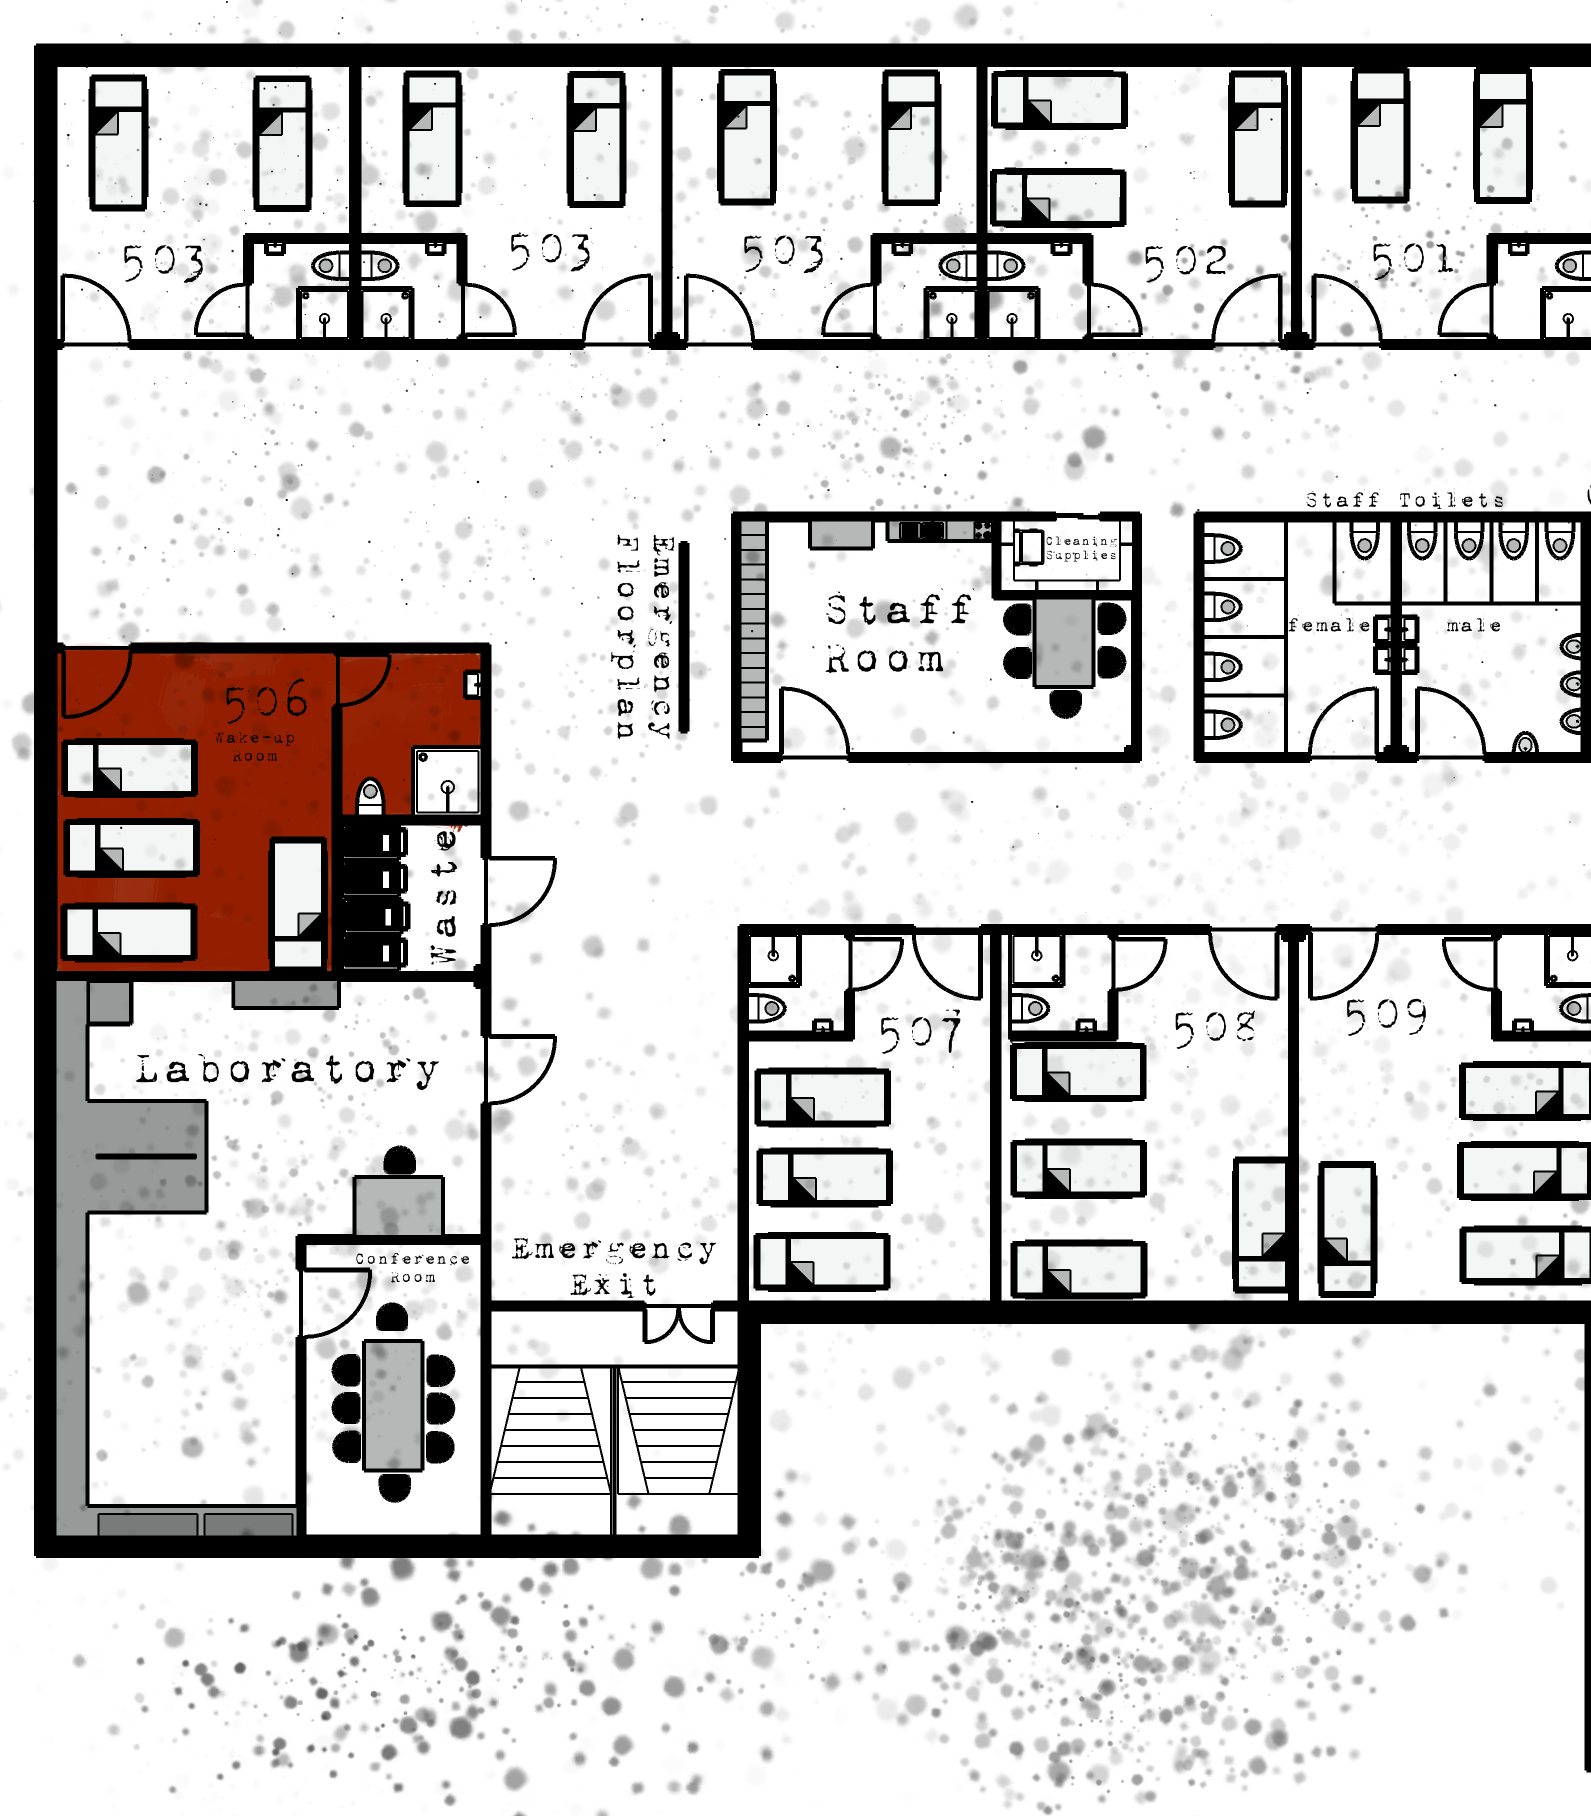
\includegraphics[width=19.5cm, keepaspectratio]{resources/img/the ward-player-L.png}
\clearpage
\onecolumn
\hspace*{-2.0cm}%
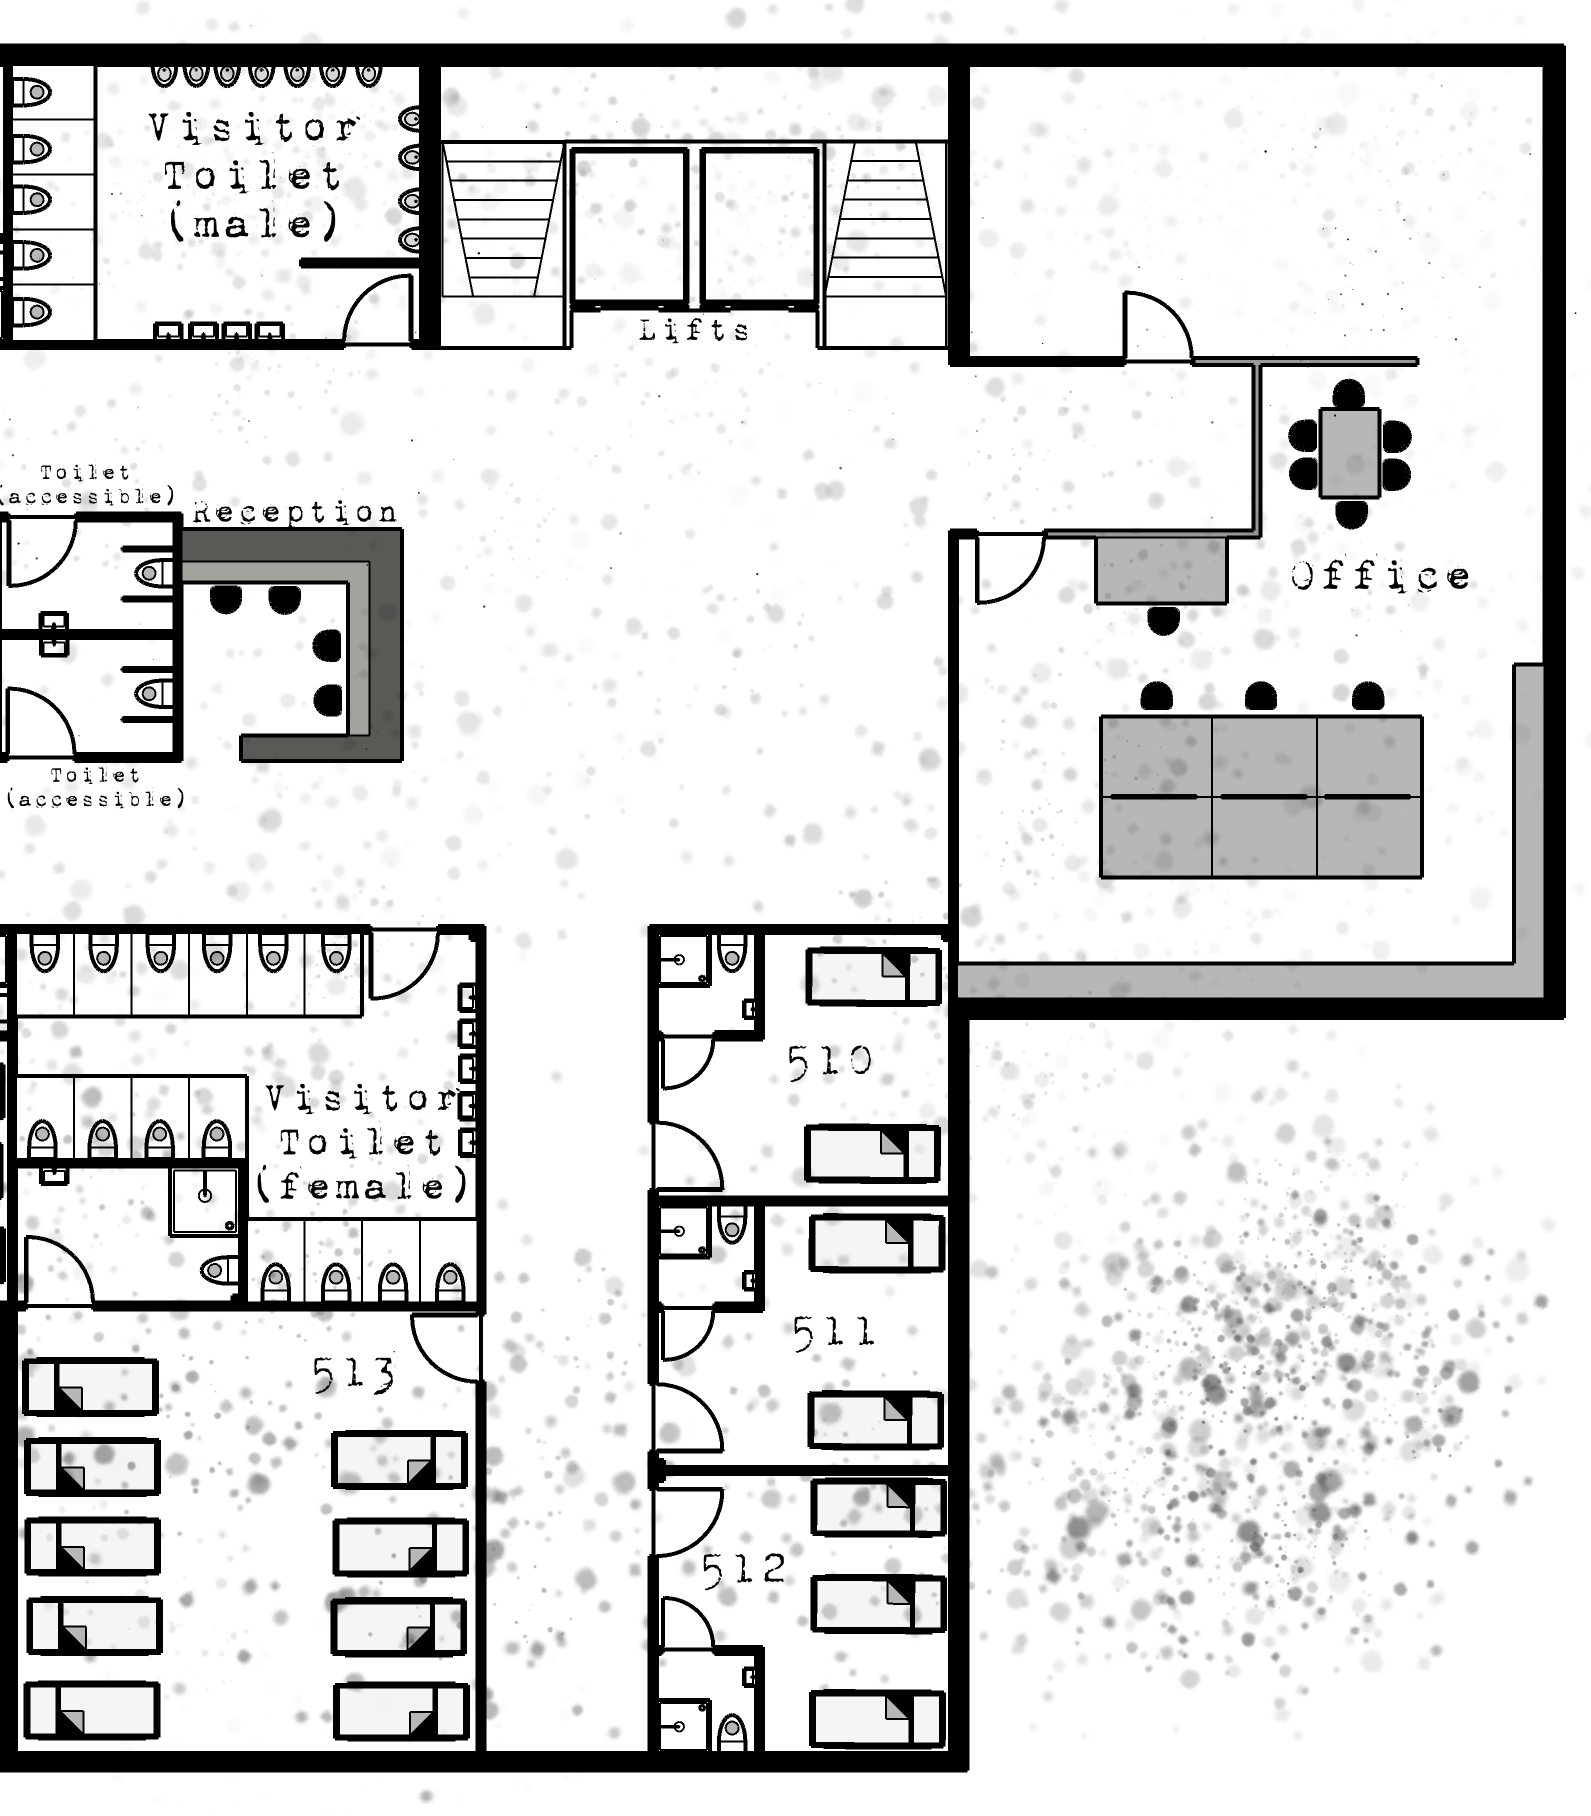
\includegraphics[width=19.5cm, keepaspectratio]{resources/img/the ward-player-R.png}
\clearpage


\onecolumn

\section{GM Section}% {{{
\label{sec:gm_section}

\subsection{About this scenario}%
\label{sub:about_this_scenario}

\subsubsection{Theme}%
\label{ssub:theme}

The theme of this scenario is life and death and the multiple things that exist in between those
extremes.
\begin{itemize}[noitemsep]
  \item The player characters start as patients in a coma, kind of at the border between life and death.

  \item \hyperref[ssub:joanna_o_banion]{Joanna O'Banion}~(p.~\pageref{ssub:joanna_o_banion}) is a vampire, obsessed with death.

  \item Dean Moran~(p.~\pageref{ssub:joanna_o_banion}) is her husband, cruel and a sociopath even before he was turned, but now
        he is in a death like sleep, which Joanna strives to wake him up from.

  \item The other patients~(p.~\pageref{ssub:other_patients}) are in a vegetative state, but their bodies can be taken by
    a wandering soul, though probably not without consequences.

  \item The orderly~(p.~\pageref{ssub:orderly}) could be a homunculus (a person grown in a jar), a zombie, or a golem created
        by Joanna to serve, a creature made from dead materials to form a pale image of something alive.
\end{itemize}

\subsubsection{Power}%
\label{ssub:power}

The death angel \textbf{Golab}~\cite[p.~215]{KULT:core} associated with the principle of torment.

They are influencing Joanna\index{O'Banion, Joanna} to do her experiments, letting her come across tomes of knowledge that
tie the spark of humanity to several different torments, misguiding her to spread more pain and
suffering to empower the death angel as well as just their enjoyment.

At the same time Golab is pushing dreams and ideas into the dormant Dean Moran\index{Moran, Dean}, who sends waves of tormented
dreams through the  ‘ether’, which mix with the characters dark secrets and cause them to re-live repressed memories,
nightmares….

Should he wake up, the first thing he will do, is devour his wife in a frenzy, thereby absorb her soul into his body, where
they will share their secrets (and those are many) and eternity.

\subsection{Using this scenario}%
\label{sub:using_this_scenario}

This scenario was made for Virtual Horror Con 2021 and should last 2--4 players about 4--5 hours including filling in the
character skeletons (see \hyperref[sec:pre_made_characters]{characters}) and some 20 minutes of chat/aftercare.

I advise you, even when you know your players, to get them to fill the
\href{https://www.gehennagaming.com/wp-content/uploads/2020/05/Gehenna-Gaming-Consent-Form.pdf}{Gehenna Gaming Consent Form}
out before the game, so you know their lines and veils and have ‘X’ and ‘O’ cards ready to react to your players needs.

See more in the fantastic~\cite{TTRPG_safety_toolkit}.

Take breaks if necessary, but also discuss with your players if this is the right game for them if there are too many red lines.

\gmnote{%
  This game is meant to frighten the characters \redbf{NOT} the players! So, please, respect their needs and wishes and tone down
  the violence/torture accordingly.  This is perfectly possible and does not make the scenario any less interesting.  I have toned
  it down for the horror con and the feedback was good.}

Thank you for running this scenario and taking this advice.

\subsubsection{Game structure}%
\label{ssub:game_structure}

The structure is fairly simple:
\begin{itemize}[noitemsep]
  \item A \hyperref[sub:coma]{setup phase} where we meet each character individually, and the players get to know their
        character.  This is one of the things I enjoy very much as it is just improvised role play, but it serves the purpose
        of having players build memories for their character, which allows them to make decisions in character more easily afterwards.

  \item The \hyperref[sub:wake_up]{wake up} where the players get to interact and discover their fate and party dynamics
        evolve.

  \item The biggest part then is the \hyperref[sub:exploration]{exploration} phase where they find out they are trapped in a
        section of the hospital they have been brought to as it is now stuck in \textbf{Inferno}.  And they are stuck with some
        orderlies of the non-human kind, a dormant vampire and one that is very much awake.

  \item The climax of the scenario is the \hyperref{sub:escape}{escape} which can either be done by one person willingly
        deciding to stay with \hyperref{sub:joanna_o_banion}{Joanna O'Banion}.  Or they find the binding circle and use that to
        their benefit.  Which still will cost them, some might get off easy, some not so much --- and some will stay behind.

  \item The ending then is again free form, where the impact of their stay in the ward and inferno is explored with each
        character.  And gives a nice circular shape to this scenario.
\end{itemize}

\subsection{NPCs}%
\label{sub:npcs}

\subsubsection{Dean Moran}%
\label{ssub:dean_moran}

Dean Moran is a vampire and in torpor for the last 150 years he is a powerful and violent dreamer, so some of his dreams spill
over to the players in the ward.  If Dean wakes up it is going to be a slaughter feast as he is thirsty and mad.  First thing he
will do is to drain his wife and lover Joanna, in his blood-thirst and frenzy.  Thereby he will absorb his wife's soul, which
will keep him company for eternity or until he will meet his final death.

Driven by his insanity and the fury of the death of Joanna he will go out and hunt the players, to empty them and use them as a
vessel for his wife's soul.

Dean Moran has been asleep for years and been alive for several centuries, his behaviour and this thoughts and speech is
inhuman, he forgot to pretend to breathe, move his eyes involuntarily, when he stands still it is like a statue.  He does not
care about his captive's integrity both mentally or physically, he will bite a finger off or break a bone just to make a point.

He is clothed in an elegant suit that was fashionable turn of the century --- 16th century that is, he sailed to the new world
when Francis Drake was fighting the Spanish armada.  Came to the new world and  driven by greed and a sense of “honour”, that
borders madness, he slaughtered both native inhabitants as well as fellow conquerors.  Back then he went by the name Alessandro
Girardi, a name that is forgotten to everyone but him.  Bested in a duel and mortally wounded he was found by someone or rather
something, he made a pact, paying with the majority of his sanity and the ability to ever see the sun again.

\paragraph{\(\diamond\)~Combat[2]}%
\begin{itemize}[noitemsep]
  \item Knock over [+0]
  \item Punch [+1]
  \item Bite [+1] (heals 1 point)
  \item Can transform his hands into claws [+2]
\end{itemize}
Dean Moran will fight ruthlessly, intelligently and dirty.
Protecting himself with the body of PC or NPC, while drinking from them.
Using cover and his environment to his advantage.
\KULTrule%

Health: \checkbox{dean-health-1} \checkbox{dean-health-2} \checkbox{dean-health-3} \checkbox{dean-health-4}
\checkbox{dean-health-5} \checkbox{dean-health-6} \checkbox{dean-health-7} \checkbox{dean-health-8}

\begin{itemize}[noitemsep]
  \item Pretend to be injured, to lure the players to come closer.
  \item Taunts and mocks players
  \item Starts looking for escape routes while fighting.
  \item Actively flees from this fight.
  \item While previously none of his wounds would bleed, suddenly all of them erupt with black ichor and white,
    writhing maggots, which feed off his blood and start growing fast.  Roll to \bluebf{Keep it Together (+Willpower)}
  \item He only flails in a last frenzy allow players to roll with \redbf{+1 Reflexes} to \bluebf{Avoid Harm (+Reflexes)} on
    his last attacks.
  \item[\KULTgold{\skull}] Falls back into the eternal sleep, if players \bluebf{See Through the Illusion (+Soul)} they will
        hear and see the souls of everyone he killed happily see him return and his soul screaming in a silent scream.
\end{itemize}

\subsubsection{Joanna O'Banion}%
\label{ssub:joanna_o_banion}

Joanna O'Banion is a vampire and has been in Chicago since the days of Al Capone, travelling with her husbands corpse in hope
of a cure for his state of torpor.  She makes detailed notes about her “experiments” some in the regular patient's file, but
the more esoteric results go in a small brown \hyperref[notebook]{notebook}~(p.~\pageref{notebook}).  Al Capone helped her
acquire a tome of alchemical formulae that speak of “torments” that might help to fill a soul into a created being.  By now she
has mastered to create homunculi, zombies, and golems of ash, clay, and other materials.  She has spoken to the spirits left by
the deceased, but the one goal she has tried to achieve for over 150 years is still not within her grasp.  She is desperate and
trying to apply the knowledge of torments and alchemy to comatose patients, in the hope to use this magic to finally wake up
Dean.

In search of people to experiment on and a corresponding control group many of those patients she has directly or indirectly
caused to be comatose.  Some of the patients might start remembering the accident they were in and seeing the orderly or Joanna
herself.

Her constant experimentation has brought the 5\textsuperscript{th} floor of Chicago central hospital closer and closer to
\textbf{Inferno}~\cite[p.~314]{KULT:core}, by successfully waking up the protagonists the floor is now completely embedded in
\textbf{Inferno}, she has managed to seal the floor off to its denizens, by barricading all entrances and exits but those
barriers are unstable and “glitchy”, i.e.~if for example a chair is taken from the barrier an exact copy will re-appear in the
barricade, with all scratches, scribbling and stuck on chewing gums.  On the other hand those barricades might also disappear
for a second or two and let in a denizen of Inferno or Limbo.

Joanna looks like a pale Italian diva from the prohibition area “costumed” as a medical doctor.  She enjoys her “research”, but
she is getting more desperate since she knows she is now stuck in Inferno and cannot get new patients and has to do with the
existing “stock”.

She will ignore the protagonists, and work on waking up Dean, unless they enter her office or make loud noises nearby (her office
doors are padded but not soundproof - so she will react to a fight or gunshots, but probably nothing less than that). When she
gets out she will try to get one or more of them to stay with her and Dean as a plaything, to play cat and mouse/hide and seek -
to satisfy her promise to study torments (worshipping Golab). Obviously not telling them the latter bit, but lying through her
pretty teeth.

\gmnote{%
  The following magic section is untested I just thought it would be cool for Joanna to be able to summon something, but during
  playtesting it never came up. What I did though is have the~\hyperref[sub:the_careerist]{careerist}, who has the
  disadvantage~\hyperref[disadv:marked]{Marked} taste her blood when attacking her and becoming a vampire when they manage to get
  out.
}

\paragraph{\(\diamond\)~Magic[2]}%
\begin{description}[noitemsep]
  \item[Summon a Spectre] A spectre is pulled from the fabric of inferno, players~\bluebf{roll to Keep it together (Willpower)}:
    \begin{description}[noitemsep]
      \item[(\KULTred{15+})] You keep your wits.
      \item[(\KULTred{10--14})] You hesitate for a moment (\redbf{-1} on next roll)
      \item[(\KULTred{-9})] You panic and freeze (\redbf{-1} ongoing until the spectre is killed).
    \end{description}
  \item[Manifest a Spectre] A called spectre (\bluebf{2 Health}) is sent off to find a dead or unconscious body and will
    express all its anger and pain from being ripped into existence, in a rampage.  It will attack randomly anything except for
    its master dealing \redbf{2 Harm}, with sharp claws.  When destroyed it turns back into spectral form.
\end{description}
\paragraph{\(\diamond\)~Combat[1]}%
\begin{itemize}[noitemsep]
  \item Knock over [+0]
  \item Punch [+1]
  \item Painful bite [+1] (heals her for 1 point) --- \bluebf{roll to Keep it together (+Willpower)}
\end{itemize}
Joanna will fight only if her life is threatened she will use whatever minion she can conjure up
\KULTrule%

Health: \checkbox{joanna-health-1} \checkbox{joanna-health-2} \checkbox{joanna-health-3} \checkbox{joanna-health-4}
\checkbox{joanna-health-5} \checkbox{joanna-health-6} \checkbox{joanna-health-7} \checkbox{joanna-health-8}

\begin{itemize}[noitemsep]
  \item Pretend to be injured, to lure the players to come closer.
  \item Taunts and mocks players
  \item Starts looking for escape routes while fighting.
  \item Actively flees from this fight.
  \item Suddenly all her wounds erupt with black ichor and writhing maggots feeding on the blood and growing fast.  Roll to
    \bluebf{Keep it Together (+Willpower)}
  \item He only flails in a last frenzy allow players to roll \redbf{+1 Reflexes} to \bluebf{Avoid Harm (+Reflexes)}
  \item[\KULTgold{\skull}] Falls back into the eternal sleep, if players \bluebf{See Through the Illusion (+Soul)} they will
        hear and see the souls of everyone he killed happily see him return and his soul screaming in a silent scream.
\end{itemize}

\subsubsection{Orderly}%
\label{ssub:orderly}
The orderly is a construct created by Joanna, to practise her necromantic arts as well as to have a servant to help her with
the maintenance of the ward. It is patrolling the ward pushing a projection or ghost of Dean around in an antique wheelchair.
Dean is only showing up when the chair is moving, appearing in his military officer attire he used to wear when he was alive.

\begin{description}
  \item[Golem] I am usually running the orderly as a golem made from graveyard earth, cigarette butts held together by fat she got from
    liposuctions done in the hospital all of that stuffed into the skin-hull of Benjamin K. Miller.  When it is killed the body
    just falls apart and a sheet of parchment buried inside the head with Hebrew writing is revealed.

    It looks like are a big burly “person” kind of ex-football player or mob enforcer.  Where in Elysium it just smells strongly of
    cigarettes, and has yellow fingers and doughy wobbly skin.  In inferno it is reeking of smoke and fat that has been in the
    fryer for way too long, and the protagonists smell it before they see it.

  \item[Homunculus] If you run the orderly as a homunculus, I would make the appearance misshapen with a big head no hair and a
    transparent skin showing the equally misshapen inner organs in Inferno.  In Elysium just a bit of wet bloated skin and
    the smell of formaldehyde.  He is grown from the organs of Benjamin K. Miller and there are several other jars of
    “Benjamins” growing in the office.

  \item[Zombie] For a zombie Joanna could have gotten them from the morgue in the basement or the graveyard of the nearby church.
    In Elysium it would just have sunken eyes and very, very bad teeth and making a sloshing sound whenever it walks (because
    of its decaying inner organs).  In Inferno go ham with zombie description, be it Walking Dead inspired or Dead Space.  And
    ask for a roll to ~\bluebf{Keep it Together (+Willpower)} to fight (on a success), hesitate (on a mixed success), or be
    paralysed or flee (player's choice) (on a failure).

    Benjamin K. Miller once found Joanna torturing a comatose patient, confronted her and didn't survive that, and now has to serve her.
\end{description}

\gmnote{
  I usually role play this NPC speaking only a very limited vocabulary and not very understandable with squawking voice, inhaling while speaking.
  You can use this list for inspiration.
  \begin{itemize}[noitemsep]
    \item yes
    \item no
    \item help
    \item patients
    \item rooms
    \item hurt
    \item doctor
    \item alarm
  \end{itemize}
}

\paragraph{\(\diamond\)~Combat[2]}%
\begin{itemize}[noitemsep]
  \item Hook punch [+1]
  \item Overhead hammer-fist blow [+2]
\end{itemize}
The orderly is very slow so any action the players do to outmaneuver or adding some other advantage should give them \bluebf{+1 to Avoid Harm (Reflexes)}.
\gmnote{When I run the Golem version of the orderly dealing 2 Harm to the head will remove the sheet of paper animating them and
finishing off the fight early.}

Health: \checkbox{orderly-health-1} \checkbox{orderly-health-2} \checkbox{orderly-health-3}

\begin{itemize}[noitemsep]
  \item Attack ignoring all wounds
  \item Shouting “alarm” unless the characters dispose of it quickly
  \item[\KULTgold{\skull}] The body falls down dead on the floor decomposing immediately.  Roll to \bluebf{Keep it Together
    (+Willpower)}.
\end{itemize}

If the characters flee and hide, it will keep searching for a bit on the corridors only following into a room if it sees them
hide in one or if the PCs made a lot of noise.

\subsubsection{Other Patients}%
\label{ssub:other_patients}

\gmnote{
  This list of patients was generated with the help of ChatGPT, and then edited, regardless of its creation: Please read
  through the list of causes and change them if you have the feeling some of them don't fit your table.  Note that there are
  duplicate of causes in there, which is intentional, some of the cases act as control group, where Joanna would experiment on
  one but not on the other!
}

\paragraph{Room 501}%
\begin{description}
  \item[Alice Harper] 32, female, pale complexion with long black hair. She ended up in a coma after a car accident caused by a drunk driver. Profession: Architect.
  \item[David Sullivan] 45, male, bald with a scruffy beard. He fell into a coma due to a severe head injury sustained during a construction accident. Profession: Construction worker.
\end{description}

\begin{description}
  \item[Room 502]
    \begin{description}
      \item[Emma Reynolds] 19, female, petite with short blonde hair. She slipped into a coma after a drug overdose. Profession: Student.
      \item[Michael Thompson] 58, male, balding with glasses. He ended up in a coma following a stroke. Profession: Accountant.
      \item[Sarah Miller] 37, female, athletic build with auburn hair. She fell into a coma after a near-fatal drowning incident. Profession: Lifeguard.
    \end{description}
  \item[Room 503]
      \paragraph{Ahmed Al-Mansour} 50, male, Middle Eastern appearance with a salt-and-pepper beard. He slipped into a coma after performing an exorcism. Profession: Priest.
      \paragraph{Yumi Nakamura} 55, female, Asian descent with elegant attire. She fell into a coma after being poisoned at a political event. Profession: Politician.
  \item[Room 505]
    \begin{description}
      \item[Lily Thompson] 23, female, petite with long red hair. She ended up in a coma after a severe allergic reaction to medication. Profession: Pharmacist.
      \item[James Anderson] 42, male, muscular build with tattoos. He mysteriously collapsed and fell into a coma during a bank robbery attempt. Profession: Criminal.
      \item[Emily Carter] 28, female, pale with dark circles under her eyes. She slipped into a coma due to extreme exhaustion and sleep deprivation. Profession: Journalist.
    \end{description}
  \item[Room 506]
    \begin{description}
      \item[Henry Wilson] 60, male, gray-haired with a kind face. He ended up in a coma after a heart attack. Profession: Retired.
      \item[Olivia Bennett] 25, female, slim with short brown hair. She fell into a coma after being exposed to a toxic substance in her laboratory. Profession: Biologist.
      \item[Benjamin Reed] 34, male, bearded with a tired expression. He slipped into a coma after a car accident caused by falling asleep at the wheel. Profession: Truck driver.
      \item[Sarah Collins] 27, female, athletic build with a nose piercing. She fell into a coma after a severe electric shock accident. Profession: Electrician.
    \end{description}
  \item[Room 507]
    \begin{description}
      \item[Maria Santos] 52, female, from the Philippines. She fell into a coma after suicide attempt. Profession: Businesswoman.
      \item[Rebecca Foster] 30, female, stylish with dyed purple hair. She ended up in a coma due to complications during plastic surgery. Profession: Model.
      \item[Daniel Hayes] 48, male, rugged appearance with a scar on his cheek. He fell into a coma after being attacked and severely beaten, protecting a client. Profession: Bodyguard.
    \end{description}
  \item[Room 508]
    \begin{description}
      \item[Mikhail Ivanov] 65, male, Russian accent with a grizzled appearance. He fell into a coma after a severe stroke. Profession: Retired.
      \item[Sarah Davis] 57, female, overweight with curly gray hair. She slipped into a coma after complications during stomach surgery. Profession: Waitress.
      \item[Christopher Nguyen] 13, male, thin and pale. He ended up in a coma after a severe asthma attack. Profession: Student.
      \item[Anna Petrov] 24, female, Slavic features with a scar on her arm. She fell into a coma after a car accident caused by reckless driving. Profession: Athlete.
    \end{description}
  \item[Room 509]
    \begin{description}
      \item[Matthew Anderson] 31, male, muscular build with a shaved head. He slipped into a coma after a drug overdose. Profession: Police officer.
      \item[Laura Miller] 39, female, petite with long brown hair. She ended up in a coma after a traumatic brain injury sustained in a domestic violence incident. Profession: Teacher.
    \end{description}
  \item[Room 510]
    \begin{description}
      \item[Mei Chen] 43, female, gentle demeanor. She ended up in a coma after a severe allergic reaction to medication. Profession: Pharmacist.
      \item[Emily White] 55, female, gray-haired with a warm smile. She slipped into a coma after a heart attack. Profession: Retired.
    \end{description}
  \item[Room 511]
    This room is empty, but there are traces of the orderly on one bed.
\end{description}


\clearpage % }}}
\section{The Story}% {{{
\label{sec:the_story}

\subsection{Coma}%
\label{sub:coma}

\subsubsection{Getting to know the characters}%
\label{ssub:getting_to_know_the_characters}

The goal of this scene is to give each player a few minutes to get to know their own character, and build some “memories”, such
that they could start the first group scene with more confidence.  In addition this scene will be giving them someone to lose
and/or care about in the world when they are brought into \textbf{Inferno}.

This scene is a one on one scene, so if you're playing face to face, ask them to sit in a chair opposite of you for the
duration of the scene; or if you're playing online ask all the other players to turn off their camera, to make the scene feel
more intense and intimate.

The scene starts with the character in coma, they don't need to know how they got in it.  The important fact is that they are
here, and with them is their important relationship who is visiting regularly, how regular is not important.  Tell the player
that because they know each other so well, as if by magic their relationship can hear their thoughts as if they were speaking
out loud.  A lot of this scene will be improvising on the spot.

If you have time enough (4h or more) this should have the following arc:
\begin{enumerate}
  \item Roll to~\bluebf{Keep it together (+Willpower)} to see how much their time in a coma has worn down their stability.

  \item The relationship tells about their current life, events that have happened in the last week, maybe small problems turn up.

  \item The relationship tells of something exciting happening, here get creative the only thing to avoid is things like a
        lottery win or other gain of wealth, because it will work against one of the goals of the introductory section to make the
        decision to accept the experimental treatment a bit more convincing.  For example things that I used were a gay couple going
        through with their adoption, a mother finding a good new potential partner, who is treating them well, sister going from doing
        bad at school to discovering a new subject that they are really good at.  This high is meant to make the next bit more dire.

  \item Since this is set in a US hospital the costs of being in there are ramping up, and for the scientist a promising new
        grant could be gotten, and similar for the careerist a new contract is in sight, if they were there to help the other
        (incompetent) team members to get that.  In essence there is the need to wake up, rather sooner than later.

  \item Last bit is to present them with a consent sheet that their relationship found or someone called in a last big favour
        to get them on an experimental treatment program, or blackmail by their relationship of the doctors here, are just a few
        examples.  Names like Joanna O'Banion\index{O'Banion, Joanna} and her expertise can be dropped, but all interactions are
        with her assistants or other doctors in this department.

  \item Ultimately the sheet is signed or the patient is put on the experimental program through favours, bribing, blackmailing
        depending what the character or rather their relationship is willing to do.

  \item After that the character is brought to the 5\textsuperscript{th} by a brutish looking orderly, with dirty fingernails
        smelling of ashes and mould.  The room (504) slowly fills with all the player characters.
\end{enumerate}

\gmnote{%
  If one of your players decides to convince their relationship to mercy-kill them, then that is perfectly fine.

  That player wouldn't wake up in the shared “wake-up room”, but in a room next door as a ghost, being able to see though walls
  as if they were semi-transparent, like frosted glass.  Dying and waking up from the dead as a ghost is a traumatic experience,
  so they loose \redbf{-2 Stability} and if the GM sees fit they gain the following disadvantage.
}

\paragraph{\(\diamond\)~\index{Disadvantages!Cannibalism}Cannibalism}\label{disadv:cannibalism}%
You have an unnatural hunger you crave for human meat whenever you see an open wound or organs roll \bluebf{Disadvantage (+0)}.
\begin{description}
  \item[(\KULTred{15+})] You are in check of your hunger, you can control it and not the other way around.
  \item[(\KULTred{10--14})] You control your hunger, but you reveal some of your urges.
  \item[(\KULTred{-9})] Your hunger is overbearing you chomp down on the feast in front of you.
\end{description}
\KULTrule%

This set of scenes is something all my players have highlighted as very intimate and enjoyable, so I wouldn't skip this.

\subsection*{Optional: wake up timer}
If you want to hone in on the impending doom and hammer home that this game is on a timer, you can periodically “broadcast”
nightmares and visions triggered by Dean Moran's\index{Moran, Dean} waking by Joanna, who is now rushing to do the same ritual
with Dean as she did with our lovely PCs.

\subsection{Wake up}%
\label{sub:wake_up}

After the patients have been brought up to the ward, there is a drastic change in tone.  The visitations of their close relations
stop visiting triggering another~\bluebf{Keep it together (+Willpower)} roll, as this should feel like a significant loss.

Instead of them a pale faced, Italian looking lady in white coat and a name tag reading Dr.~O'Banion.  She experiments on them
noting the results in \hyperref[notebook]{a worn notebook}~(p.~\pageref{notebook}). Those experiments are inhumane, suffocation,
cutting, electrocution, and tattooing something on their backs. Note that the protagonists are unable to see or everything in
detail so the smell, sound, and other sensations should give a some horror of not knowing exactly what happened. The protagonists
can later learn about this in the patient files at the foot of their beds.

\subsection{Exploration}%
\label{sub:exploration}

The constant experimentation of Joanna O'Banion\index{O'Banion, Joanna} has brought the 5\textsuperscript{th} floor of Chicago
central hospital very close to \textbf{Inferno}~\cite[p.~314]{KULT:core}.  By successfully waking up the protagonists the floor
is now completely embedded in \textbf{Inferno}, she has managed to seal the floor off to its denizens, by barricading all
entrances and exits but those barriers are unstable and “glitchy”.

In general the \textbf{Illusion} in the ward is thin enough that if you try to \bluebf{See Through the Illusion} you see back
into “Reality”, and you can see the mundane life in a regular hospital, or just hear muffled sounds or smells on a success with
complications.

\subsubsection{Wake-up room: 504}%
\label{ssub:wake_up_room}

\begin{figure}[!htbp]
  \centering
  \includegraphics[width=7.0cm, keepaspectratio]{resources/img/wakeup-room.png}%
  \caption{Wakeup Room}
\end{figure}

This is where our protagonists are being brought to from the third floor and then subsequently wake up. First just feeling a
tingle in their body which goes away and then a wave hits all of them (triggered by Joanna starting to experiment on Dean, and
torturing someone loved by her), waking them up - Golab wants to disrupt her experiments, to make her more miserable.Joanna is
somewhat aware that something happened but focusses on "waking up" Dean. Surprisingly the experiments have reversed the muscular
atrophy and the protagonists feel quite healthy despite having been in a coma.

There is a nightstand next to everyone's bed with their regular street clothes and anything their relationship would have been
stashing in here.

There is a washing room with a toilet, shower and sink with mirror, which can be used for looking at the back to see the tattoo or
for the GM to trigger~\bluebf{Disadvantage} rolls for Nightmares or the like.

\gmnote{In one of my playtests I had a player with Nightmares, see encounter a single moth in the bathroom bumping against the
light, and later on a lot more whenever they found a reflective surface - tying the Disadvantage to the "Moth child".}

At the end of each bed is a medical file with a complete documentation of all the \textbf{medical} procedures, that includes a
\textbf{massive tattoo} in the shape of a symbol, which someone versed in lore would recognise as the symbol of the Death Angel
Golab.

\begin{figure}[!htbp]
  \centering
  
\includegraphics[width=4.0cm]{resources/img/golab.png}
  \caption{Tattoo~\cite[p.~215]{KULT:core}}
\end{figure}

\gmnote{%
  In my play-tests I had the mother of the criminal put a bottle of good red wine, cutlery and a plate and a chequered napkin
  as a improvised table cloth in there.  Letter openers, knives pen, paper, newspapers with crossword puzzles.  Basically
  anything that would have been used in the opening scene or what the archetype would plausibly have.  All mobile phones have
  just a bit of battery left and just one bar of reception, if the close relationships are asleep they can be called in
  their dreams, but there is a lot of static on the call and they will expose the person they call to the influence of
  \textbf{Inferno} or \textbf{Limbo}~\cite[p.262]{KULT:core}.

  The mirror I used with great success to let moths (foreshadowing the \textbf{Moth Child}~\cite[p.~270]{KULT:core})
  appear, since the prolonged comatose sleep has brought the patients closer to \textbf{Limbo}.%
}

\subsubsection{Corridors}%
\label{ssub:Corridors}
The corridors have neon lights with motion sensors, when they wake up everything is dark outside, and the lights turn on
wherever they walk, with that unnerving ‘\textit{tick-tick-humm}’ that neon lights tubes do.  The walls have a few art prints of
a painter named ”Guy Vauquelin”\footnote{which you can use to tie it to the published scenario “The Atrocity Exhibition”
in~\cite[p.~94]{KULT:taroticum}}, and there are some indoor plants that are surprisingly well kept and alive.  Apart from that
I always ran this as an empty hospital, but, depending on the lines and veils of your players, you can go hog wild here and add
bloodstains, debris, mutilated and corpses drained of blood, signs of fight and struggle.  And since this is a pocket of reality
inside Inferno, you can make the walls move and ripple while you hear the sound of people from the other side of the veil or
children playing on a playground from the dream of one of the still comatose patients.

\subsubsection{Lifts}%
\label{ssub:lifts}

They will fall into their shafts the first time they are visited door closes, and then they reappear as if nothing happened
roll to \bluebf{Keep it Together (+Willpower)}.

If player's try to use them they will just fall through the floor.  Let them roll to \bluebf{Avoid Harm (+Reflexes)} to catch
themselves.  If they fail, they will fall down and back into the lift on the 5\textsuperscript{th} floor (because space is
just an illusion) and suffer \KULTred{1 harm} which they can roll to \bluebf{Endure Injury (+Fortitude)} for.

If player's decide to climb up or down, let them roll to \bluebf{Avoid Harm (+Reflexes)}, to avoid the lift hitting them from
above.  If they fail, they will fall down same as above.

Regardless of what they do, they will always end up on floor 5.

\subsubsection{Emergency Exits (\faLock)}%
\label{ssub:emergency_exits}

All exits are barricaded and warded by \hyperref[ssub:joanna_o_banion]{Joanna O'Banion} against intruders from \textbf{Inferno}.
If players try to see through the illusion close to any exit the will see some of the citizens or the shadow of the
\textbf{Black Citadels}~\cite[p.316]{KULT:core}.

They can break off the leg of a chair or take an IV stand pole which make up the barricade as a makeshift weapon.

\subsubsection{Other patient rooms: 503}%
\label{ssub:other_patient_rooms_503}

\subsubsection{Other patient rooms: 50x}%
\label{ssub:other_patient_rooms}
\todo[inline]{move other patients in here}
These rooms are filled with other comatose patients.  Since Joanna O'Banion is a very diligent scientist as well as a skilled
alchemist, some of the patients will share a (uncanny) likeness with our protagonists.  These are the “control group” to make
sure that scientific/alchemistic discovery is not left to coincidence and is reproducible.

If one the protagonists die they may try to roll for \bluebf(Engage in Combat (+Violence)) to take over one of those comatose
bodies.

\begin{description}
  \item[On a (\KULTred{15+})] they can occupy the new body.  For the changed physicality let them change two of their active
        attributes.
  \item[On a (\KULTred{10--14})] they can share a new body with the current soul that is in there.  I used Sophie Liu (24), a
        talented climber, who had an accident in a tour.  She's very vocal about her not liking the sharing of her body, which is
        something nobody else can hear.
  \item[On a (\KULTred{-9})] they share the body with Sophie, but they suffer another \redbf{-1 Stability}, and get a new
        disadvantage \hyperref[disadv:cannibalism]{cannibalism}~(p.~\pageref{disadv:cannibalism}).
\end{description}

In any case the tattoo found on their original body will soon show up soon Sophie's back as well.

As far as the protagonists can see the control group has endured the same \textbf{medical} procedures, but none of the
“experimental” stuff.

\subsubsection{Staff Room (\faLock)}%
\label{ssub:staff_room}

This room is locked, but the key can be found with the \hyperref[ssub:orderly]{orderly}~(p.~\pageref{ssub:orderly}).  Also the
criminal~(p.~\pageref{sub:the_criminal}) can use their advantage of \bluebf{Burglar}, or someone can try to force the door open
by \bluebf{Engaging in Combat (+Violence)}, this last option will always be loud and get the attention of the orderly.

Inside the room there is
\begin{description}
  \item[a bunch of lockers] on the left wall, the blue colour is peeling off and you can see the rust.  There is a pistol and 2
        magazines inside~(see p.~\pageref{pistol}).
  \item[a working fridge] with a big green puddle.  The door is slightly ajar and inside there is a lot of mouldy food,
        the source of the puddle, and three beautiful roses.
  \item[a old computer with CRT monitor] on it there is a bunch of snuff porn and some searches about ‘torment’, there is a
        site about gruesome deaths in the internet explorer history, as well as some scanned pages containing weird (alchemical)
        symbols.  Reason why Joanna was using this computer for research is that only here the internet connection is working.  The
        protagonists can send emails to the outside world, but everything will take a while, and everything is old.
  \item[a kitchenette] used and some chairs and a crappy table, if someone tries to \bluebf{See through the Illusion (+Soul)}
        there are people moving through the room, staff from the other side of the veil.
\end{description}

\subsubsection{Laboratory (\faLock)}%
\label{ssub:laboratory}

The lab is a tidy room, the shelves are nicely sorted and the bottles of various chemicals are neatly labelled.  In the corner there
is a locked fridge with a glass door filled with medical samples, some of them being blood samples some filled with pale yellow liquor
samples, some of them labelled with the protagonists' names as well as some bar-code.See~(p.~\pageref{ssub:vials}) for more info on those.

In the bottom half there is a stash of opiate based pain killers requiring a \redbf{Disadvantage roll} for \redbf{Drug Addicts}, also
there is a bag of 12 black polished rocky dodecahedrons (whiskey stones).  And two bottles of white wine from 1912 with a worn label
referencing this as custom made for “RMS T\_t\_\_\_c”\footnote{RMS Titanic}.
\todo[inline]{fill me}

\subsubsection{Reception}%
\label{ssub:reception}

In my game the reception never came up as a meaningful location I kept it as a backup solution for the \textbf{staff room} so
instead of breaking open the door of the staff room I would still let the players do an \bluebf{Observe the situation (+Perception)}
or \bluebf{Investigate (+Reason)} to find the \textbf{pistol}.  There is a computer and some drawers where the protagonists might
find the \textbf{master keys/ID card}.

\subsubsection{The Office (\faLock)}%
\label{ssub:the_office}

This is where \hyperref[ssub:joanna_o_banion]{Joanna O'Banion} has her “Lair”, it is filled with a few workstations which all
don't work she has to light the office with candles, though the purple glow of the magic circle carved into the ground and
inlaid with tin does provide a bit of illumination in the back of the room.


\subsubsection{Other Rooms}%
\label{ssub:other_rooms}

\begin{itemize}[noitemsep]
  \item Toilets
  \item Waste Room (\faLock)
  \item Conference Room
  \item Cleaning Supply Room (\faLock)
\end{itemize}

These rooms are just set dressing, I have not planned anything with them, but feel free to introduce new and terrible surprises
for your players in here.

\subsection{Escape}%
\label{sub:escape}

There are two intended ways to escape from “The Ward”, adjust them to your game as needed.

\subsubsection{Option 1}%
\label{ssub:escape_option1}
One character willingly staying with Dean or Joanna will end the scenario and catapult the other characters out of
\textbf{Inferno} into their own bodies in the hospital, but not to the comatose ward from the opening scene, but one floor
above where they were brought to, which is now a regular sleep study station.  They are standing around clad in hospital gown,
where the nearest doctor or nurse will notice them and bring them to their room one floor below, which they have apparently
never left.

\subsubsection{Option 2}%
\label{ssub:escape_option2}
There is a binding circle in the laboratory.  The room is locked, but the door can be forced open or the PCs can use the staff
keys found on the \hyperref[ssub:orderly]{orderly}.  Stepping into the circle without preparation will cause its magic to
violently interact with the magic of the binding circle on the PCs back, dealing \KULTred{3 Harm} to \bluebf{Endure Injury
  (+Fortitude)}.  Using whatever they find in the lab or otherwise they can try to roll \bluebf{Engage in Combat (+Violence)} to
destroy the circle.

\begin{description}
  \item[On a (\KULTred{15+})] they will escape successfully.
  \item[On a (\KULTred{10--14})] there is a price to be paid, they leave something behind.
  \item[On a (\KULTred{-9})] the GM chooses one of
        \begin{itemize}[noitemsep]
          \item they cannot escape and have to stay as the pet of Joanna and Dean.
          \item they leave their body in \textbf{Inferno}, but return as a disembodied soul.
          \item they have to exchange someone from \textbf{Elysium}~\cite[p.~224]{KULT:core} to take their position here.
        \end{itemize}
\end{description}

\subsection{Home}%
\label{sub:home}

To close this scenario and tie in with the opening scene, I end the game with an improvised scene playing one year after the
last scene.  You can tie in the personal relations and extrapolate what might have happened to them in a year after the wake up.
In my play tests I made the relation of the people who stayed behind, start looking for clues where the PC went.  Ultimately
seeking out the other PCs for help, or explanation, after all they were also comatose in the same ward.

Characters who were left behind will be playing a game of cat and mouse with Dean\index{Moran, Dean}, maybe getting killed and
resurrected just to be chased and tortured another day, you can hint that they managed to escape \textbf{Inferno} after a few
years.

\clearpage % }}}
\section{Objects and Maps}% {{{
\label{sec:objects_and_maps}

\twocolumn
\subsection{Objects}%
\label{sub:objects}

\subsubsection{Keycard}%
\label{ssub:keycard}

The orderly has a \textbf{keycard} that opens every locked door in the ward.
\begin{figure}[!htbp]
  
\includegraphics[height=5.5cm, keepaspectratio]{resources/img/keycard.png}
  \caption{Orderly's keycard}\label{keycard}
\end{figure}

\subsubsection{Pistol}%
\label{ssub:pistol}

\begin{figure}[!htbp]
  
\includegraphics[width=5.5cm, keepaspectratio]{resources/img/glock.png}
  \caption{Pistol found in the only locked locker in the \textbf{staff room}}\label{pistol}
\end{figure}
The gun belonged to the security guard, before he was turned into what he is now.  There is also a driver's license in the
locker belonging to a Benjamin K. Miller, and the photo shows someone very similar looking to the
\hyperref[ssub:orderly]{orderly}, less bloated and grey though.


\subsubsection{Vials}%
\label{ssub:vials}

\begin{figure}[!htbp]
  \centering
  
\includegraphics[width=5.5cm, keepaspectratio]{resources/img/test tubes.png}
  \caption{Vials of spinal fluid extracted for experimentation}\label{vials}
\end{figure}
These vials can be found in the fridge in the laboratory, four of them have their name and room number attached.  When they are
taken out and not put in a cooler they are starting to develop black flakes like ash or grime, while at the same time fingers
or toes go numb and start to blacken with necrosis.  If they are not put back into cold storage in time characters will incur
\redbf{1 Serious Wound} that can be stabilised by putting the vials in a cold place for a while.

When one of these vials is destroyed the PC named on the vial just dies instantaneously, which allows their spirit to leave the
body.  This will cost them \redbf{-2 Stability} for the traumatic experience of dying.  The PC's spirit can now try to find a new
body in one of the \hyperref[ssub:other_patient_rooms]{other patient rooms}~(p.~\pageref{ssub:other_patient_rooms}).

\subsubsection{Documents}%
\label{ssub:documents}

\begin{figure}[!htbp]
  \centering
  \includegraphics[width=5.5cm, keepaspectratio]{resources/img/journal.png}
  \caption{Joanna O'Banion's journal with the “experimental” procedures}\label{notebook}
\end{figure}

\clearpage % }}}
\onecolumn
\subsection{Map}%
\label{sub:map}
\hspace*{-0.5cm}%
\includegraphics[width=19.5cm, keepaspectratio]{resources/img/the ward-gm-L.png}
\newpage
\vspace*{0.55cm}%
\hspace*{-2.0cm}%
\includegraphics[width=19.5cm, keepaspectratio]{resources/img/the ward-gm-R.png}
\section{Credits}% {{{
\label{sec:credits}

\subsection*{Credits}

\begin{itemize}[noitemsep]
  \item My partner Andressa for always being there for me and being awesome in general.
  \item Afy for patiently answering a ton of questions about writing and mentoring me when I started writing this.
  \item Kaela for suggesting to have a wrap up and circle back to the beginning.
  \item Seth Skorkowsky for reviewing scenarios, pointing out flaws and how to make them better.  Especially his video on
        \href{https://www.youtube.com/watch?v=MGxO88C5WFI}{20 Tips for Publishing Your RPG Adventure} was a great resource.
  \item All who participated in creating~\cite{KULT:tex}.
  \item All art is made with free stock imagery from pexels.com, shutterstock.com, unsplash.com, and images in the public
        domain from wikipedia/wikimedia post processed in Inkscape, Gimp or Krita, thanks to all people developing these and
        making their photography available on those free stock image sites.
  \item The map is handmade in SketchUp with valuable feedback from my Dad.
\end{itemize}

\clearpage % }}}
\phantomsection%
\printbibliography[title={Bibliography},heading=bibintoc]
\clearpage
\printindex
\end{document}
